\section{Teil 1 Mechanik}
\label{sec:teil-1-mechianik}
\subsection{Einleitung}
\subsection{Aufgabenstellung}
\subsubsection{Zielsetzung}
\subsubsection{Problematik}
\subsection{Konzepte} \newpage

\subsubsection{Variante 1} 
\textbf{Übersicht der Prozessschritte:}
\begin{itemize}
\item[1] Füllen des Futtermagazins
\item[2] Führen zur Schneidplatte
\item[3] Schnitt
\item[4] Pressen
\item[5] Entsorgen
\item[6] Füttern
\end{itemize}

\textbf{1.Füllen des Futtermagazins:} \\

Im folgenden Bild wird mithilfe einer Lego-Darstellung gezeigt, wie das Magazin aus verschiedenen Blickwinkeln befüllt aussieht. Hier muss man beachten das die vom Hersteller zu öffneten Seite in Richtung des Schneidewerks zeigt (die schmale Seite mit der Einkerbung).

\begin{figure}[H]
\begin{center}
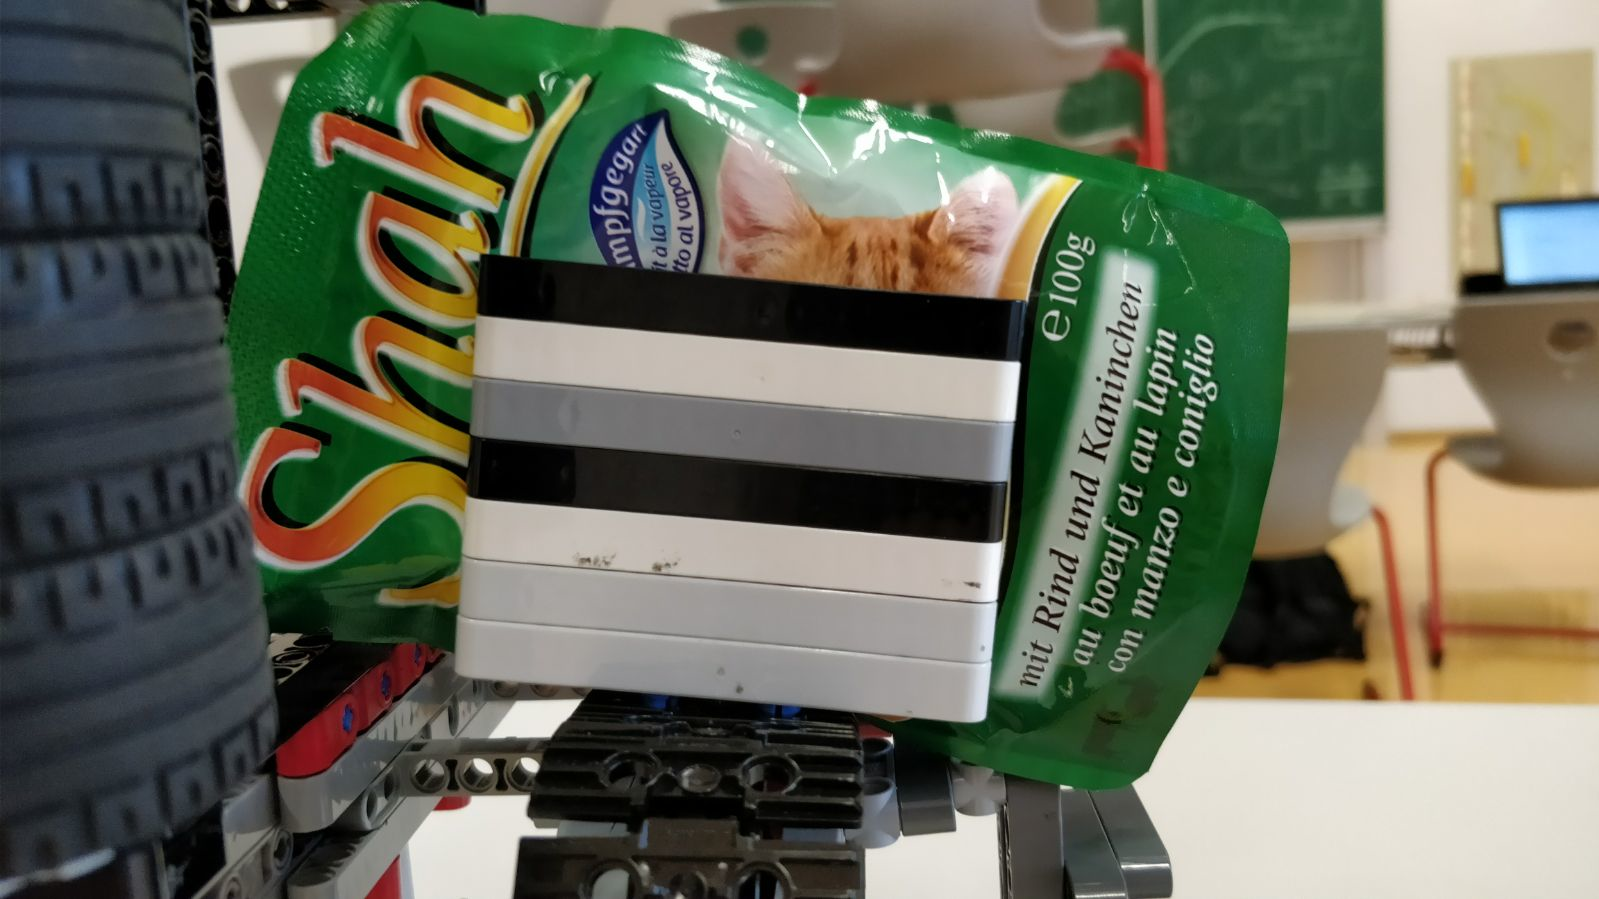
\includegraphics[width=13cm]{Bilder/Ablauf_1_png/Magazin_Vorne.png}
\caption{Magazin Vorne}
\end{center}
\end{figure}

\begin{figure}[H]
\begin{center}
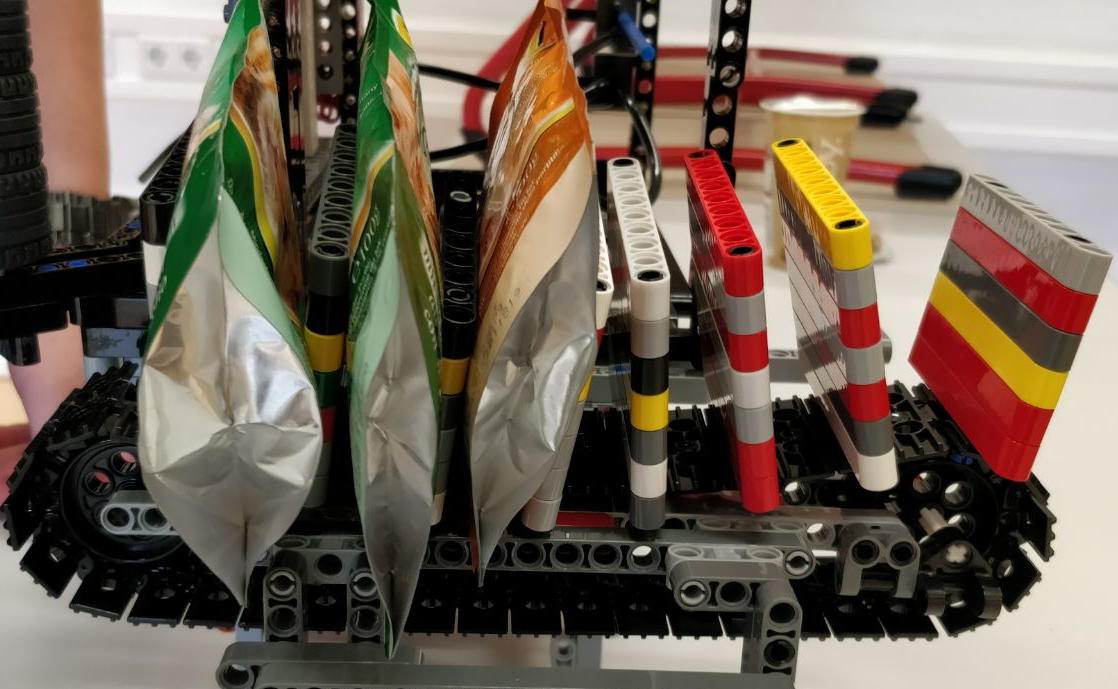
\includegraphics[width=13cm]{Bilder/Ablauf_1_png/Magazin_Seitlich.png}
\caption{Magazin Seitlich}
\end{center}
\end{figure}

\begin{figure}[H]
\begin{center}
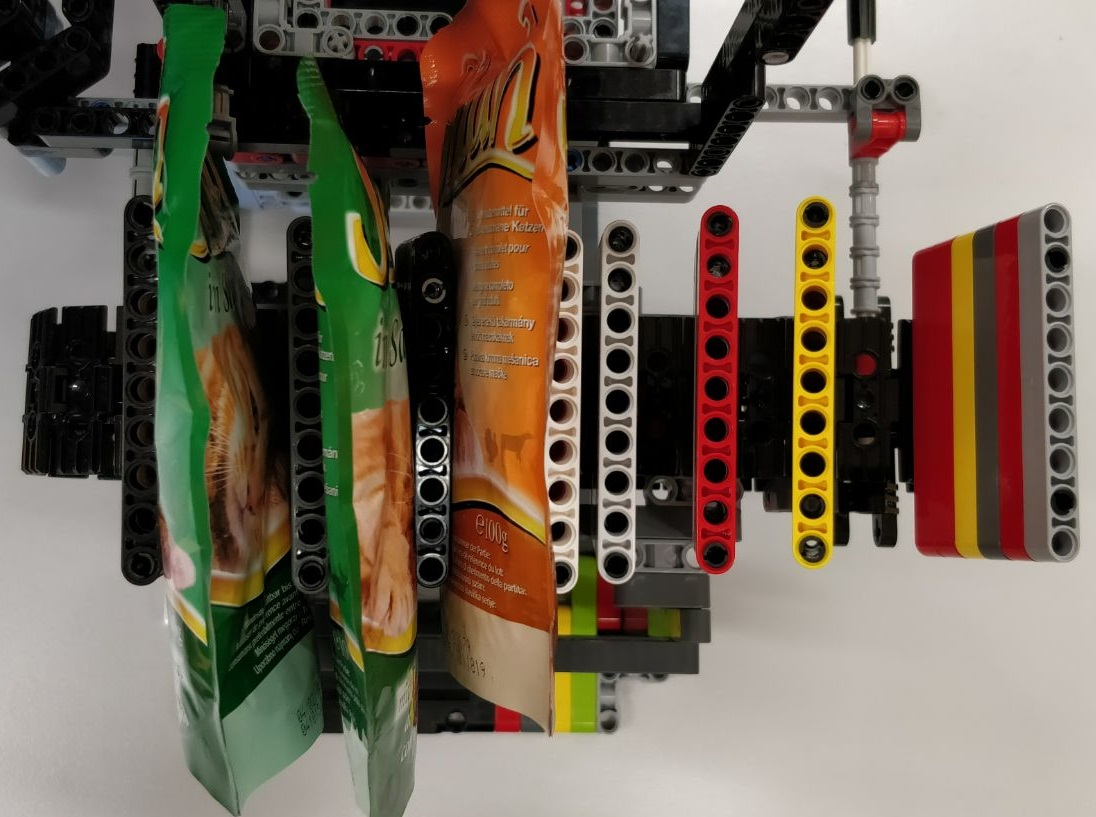
\includegraphics[width=14cm]{Bilder/Ablauf_1_png/Magazin_Oben.jpeg}
\caption{Magazin Oben}
\end{center}
\end{figure}

\newpage 

\textbf{2.Führen zur Schneidplatte:} \\ 

In diesem Schritt wird mithilfe eines Greifers (dargestellt durch eine Hand) die Packung in richtiger Position gebracht.

\begin{figure}[H]
\begin{center}
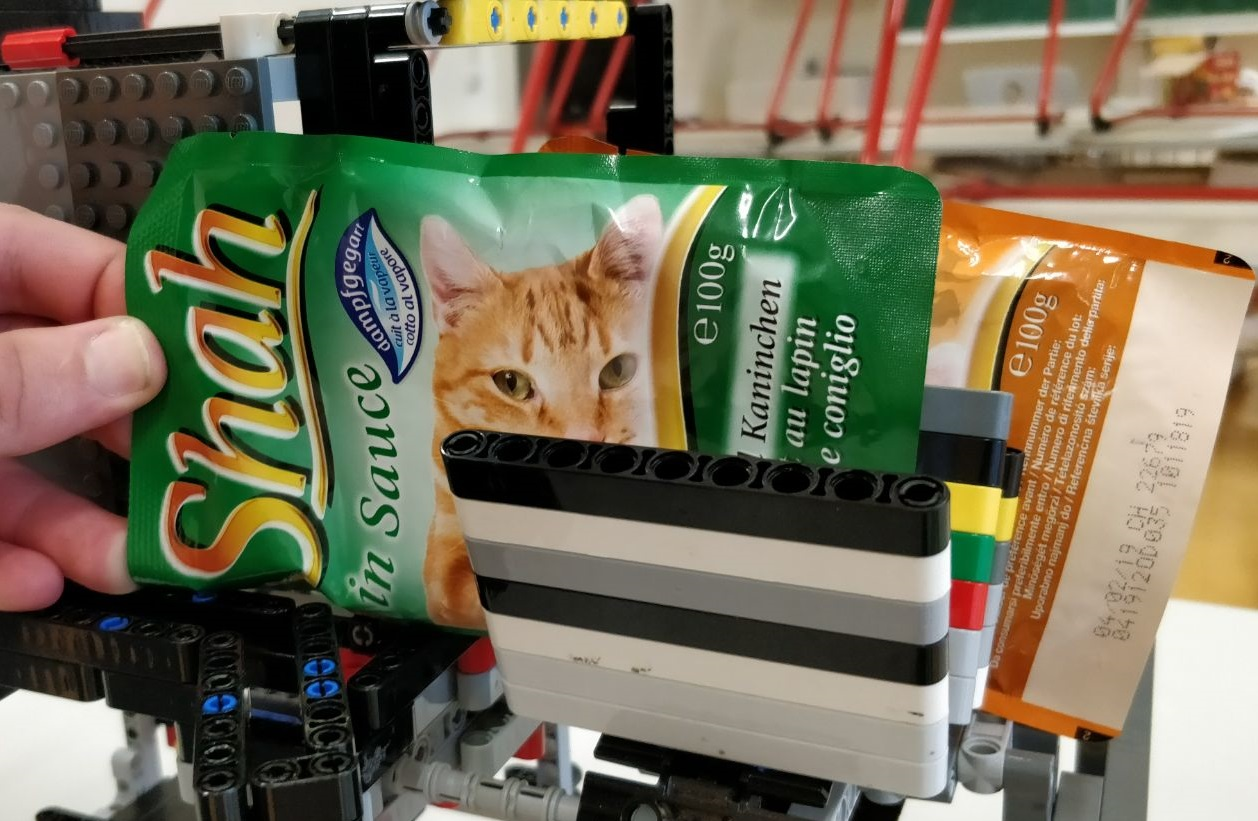
\includegraphics[width=14cm]{Bilder/Ablauf_1_png/Magazin_Auszug.jpeg}
\caption{Magazin Auszug}
\end{center}
\end{figure}

\begin{figure}[H]
\begin{center}
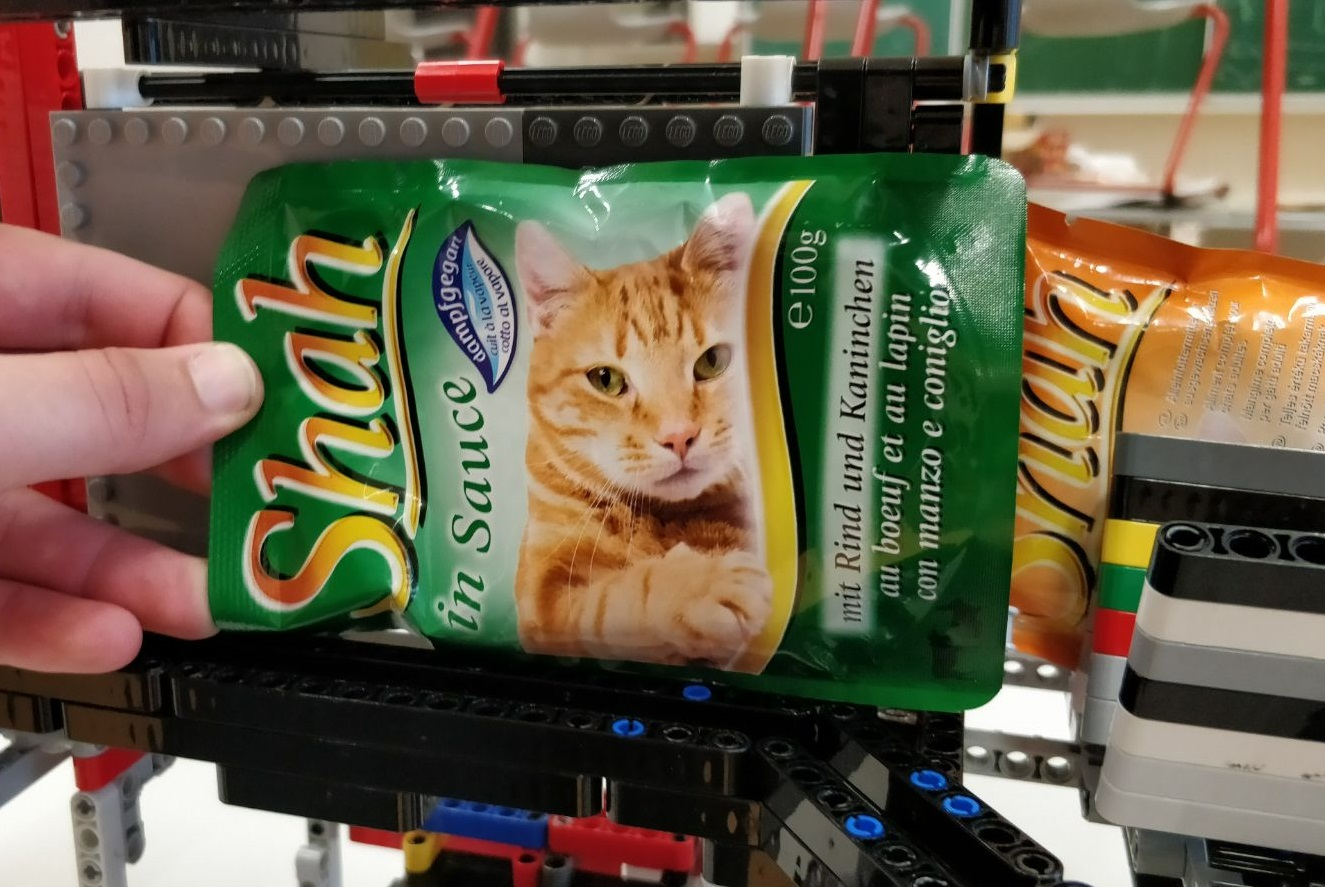
\includegraphics[width=14cm]{Bilder/Ablauf_1_png/Magazin_Auszug_2.jpeg}
\caption{Magazin Auszug 2}
\end{center}
\end{figure}

Wie im Bild gezeigt liegt das Katzenfutterpackerl in der richtigen Position und wird mit zwei Magnetzylindern an der Schneidefläche festgehalten.

\begin{figure}[H]
\begin{center}
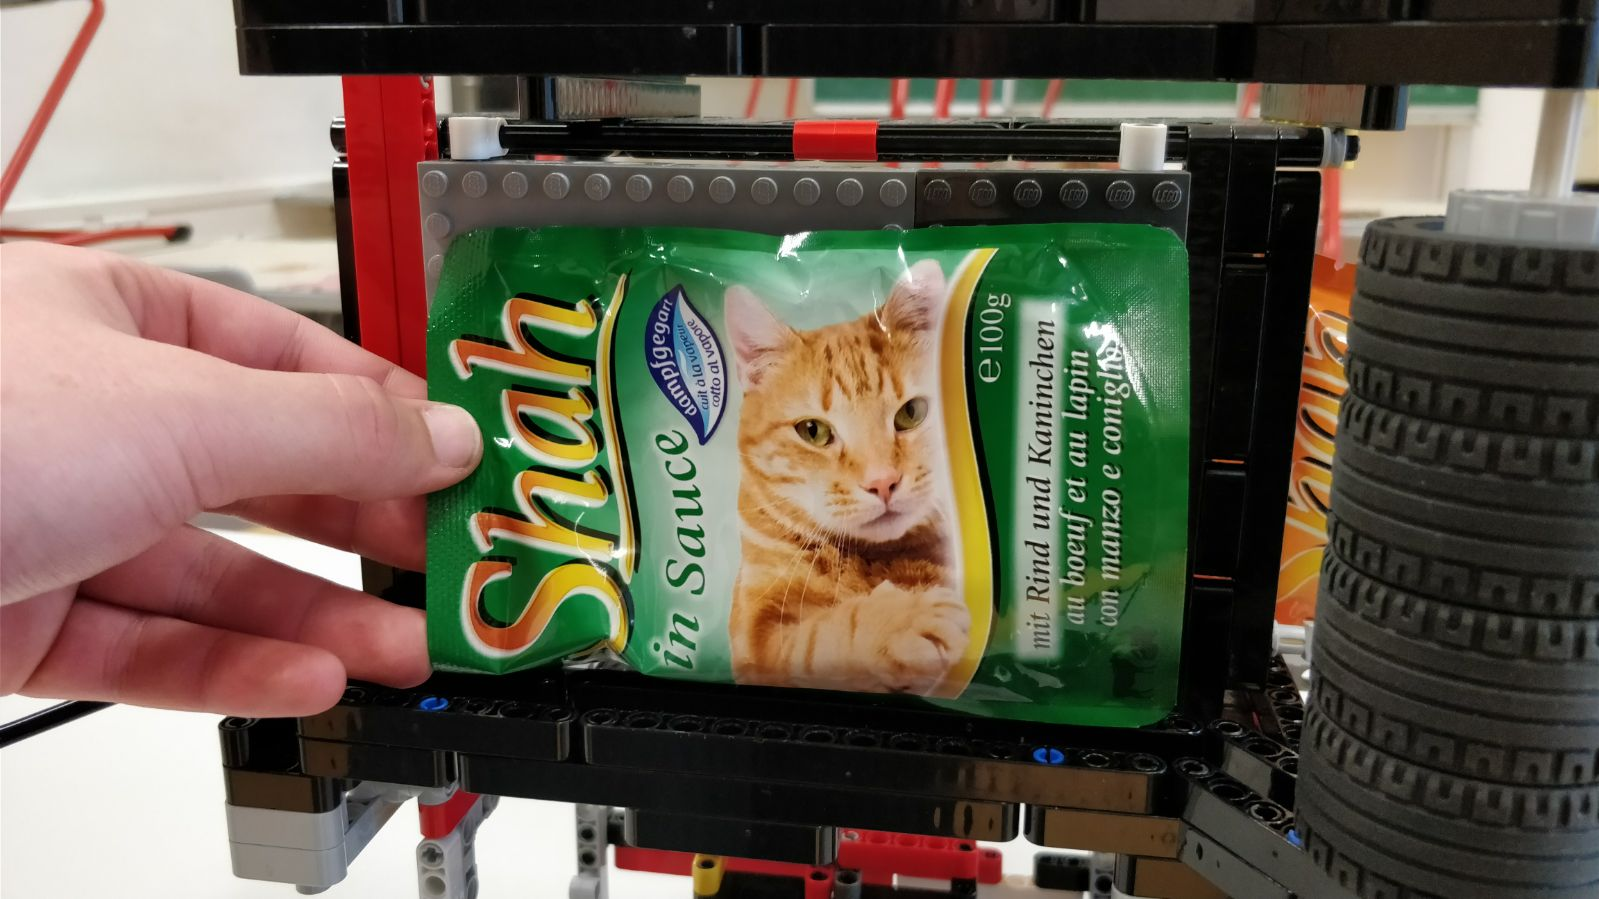
\includegraphics[width=14cm]{Bilder/Ablauf_1_png/Schneidebereit.jpeg}
\caption{Schneidebereit}
\end{center}
\end{figure}

\subsection{Aufbauten und Tests}
\subsection{Vergleich der Varianten}
\subsection{Konstruktion der Wahlvariante und Details}
\subsection{Berechnung und Dimensionierung}
\subsection{Simulation}
\subsection{Bedienung und Wartung}
\subsection{Selbstkritische Analyse und Ausblick}